\chapter{Design}

\section{Denahvit Hardenbeg}

Denahvit Hardenberg or DH, is a method to compute every joint/axis into parameters of the coordinate systems.\\
These descriptions of the system can be used to translate every point and every movement of the robotic manipulator, with the help of forward kinematic.\\
Initially the start is to locate all of the coordinate systems, as seen in \ref{fig:DH-Parameters}.\\ 
\begin{figure}[h]
    \centering
    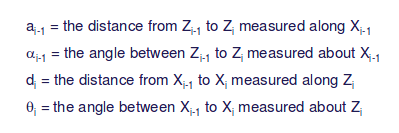
\includegraphics[scale=0.65]{Design/DH.png}
    \caption{DH-Parameters \cite{DH}} 
    \label{fig:DH-Parameters} 
\end{figure}

\newpage

Then the angles and the distance from each coordinate system is computed and set in to a table as seen in \ref{fig:DH-Table}.

\begin{figure}[h]
    \centering
    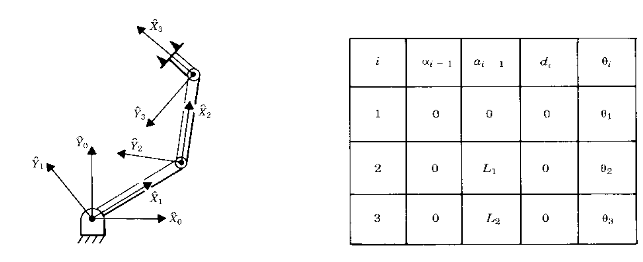
\includegraphics[scale=0.5]{Design/DH1.png}
    \caption{DH-Table \cite{DH}} 
    \label{fig:DH-Table} 
\end{figure}

As seen in \ref{fig:DH-Table},the coordinate systems is used to trace every step of each axis.\\
Starting from left to right at the top of the table, the alpha-1 is used to compute the difference between the angle between Zi and Zi-1, which is 0, due to the fact that they keep the same angle from Zi to zi-1.\\
It can also be seen from the table that the distance between Zi and Zi-1 is Length2, since they are parallel to each other.\\ 
The distance between Xi-1 and Xi is 0 since they cross each other on the perpendicular line, which means that in that point the new coordinate system should be placed.\\

